\section{Background}
\label{sec:background}

\subsection{zkML Workflow and Proving Pipeline}
\label{sec:zkml-pipeline}

As shown in Figure~\ref{fig:zkml-workflow}, a client submits an input \(x\) to a model provider, which evaluates a model with parameters \(\theta\) to produce \(y=f(x,\theta)\). The provider returns \(y\) together with a ZK-SNARK proof \(\pi\) attesting that the specified computation produced that output. Which values are public or private depends on the application.

To generate \(\pi\), the model is mapped to a proof-compatible representation, often using quantized integer or fixed-point arithmetic~\cite{boyuan2021zen,chen2024zkml}, and compiled into an arithmetic circuit or constraint system~\cite{gabizon2019plonk}. Circuit-specific proving and verification keys can be prepared ahead of time or generated on demand and reused across requests that share the same circuit configuration. For each request, the prover constructs the \emph{witness}, containing the private values required to satisfy the circuit constraints, and generates \(\pi\). The client verifies the proof using the verification key without re-executing the inference.

\begin{figure}[t]
    \centering
    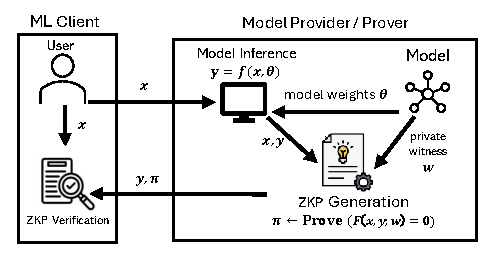
\includegraphics[width=\linewidth]{figures/background/zkInfer_workflow.pdf}
    \caption{zkML inference and verification workflow. The model provider returns an output $y$ and a proof $\pi$ attesting that $y$ was produced by evaluating the claimed model on input $x$.}
    \Description{Diagram showing a client sending an input to a machine-learning service provider. The provider evaluates a model, generates a zero-knowledge proof of correct inference, and returns the output and proof to the client, which verifies the proof.}
    \label{fig:zkml-workflow}
\end{figure}

\subsection{Proof Generation as a Systems Bottleneck}
\label{sec:proving-bottleneck}

zkML proving is substantially more expensive than ordinary model execution because the prover must demonstrate that an arithmetic constraint system is satisfied. Operations such as fixed-point arithmetic, nonlinearities, comparisons, and range checks may introduce additional constraints or lookup arguments~\cite{chen2024zkml,kang2024scaling,liu2021zkcnn}. Proof generation also materializes witness, circuit, proving-key, and polynomial data that can make the working set much larger than the model's inference activations.

These costs create systems-level constraints. Long proof times increase request latency, while large working sets restrict both the size of proof jobs that can execute on a machine and the number that can overlap safely. The problem becomes more pronounced in a serving setting, where multiple inference requests compete for finite compute and memory.

\begin{figure}[t]
\centering
\scriptsize
\begin{tikzpicture}[
op/.style={draw, rounded corners, minimum width=0.85cm, minimum height=0.42cm, align=center},
job/.style={draw, dashed, rounded corners, inner sep=4pt},
edge/.style={-{Latex[length=1.5mm]}, thick},
node distance=0.55cm and 0.75cm
]
\node[op] (x) {Input};
\node[op, right=of x] (conv) {Conv};
\node[op, right=of conv] (relu) {ReLU};
\node[op, above right=0.35cm and 0.85cm of relu] (a) {Op};
\node[op, below right=0.35cm and 0.85cm of relu] (b) {Op};
\node[op, right=2.0cm of relu] (add) {Add};
\node[op, right=of add] (y) {Output};
\draw[edge] (x) -- (conv);
\draw[edge] (conv) -- (relu);
\draw[edge] (relu) -- node[above left] {$t_1$} (a);
\draw[edge] (relu) -- node[below left] {$t_1$} (b);
\draw[edge] (a) -- node[above right] {$t_2$} (add);
\draw[edge] (b) -- node[below right] {$t_3$} (add);
\draw[edge] (add) -- (y);
\node[job, fit=(conv)(relu), label=below:{Job 1}] {};
\node[job, fit=(a), label=above:{Job 2}] {};
\node[job, fit=(b), label=below:{Job 3}] {};
\node[job, fit=(add), label=below:{Job 4}] {};
\end{tikzpicture}
\caption{Example inference graph partitioned into four proof jobs. Intermediate tensors \(t_1\), \(t_2\), and \(t_3\) cross job boundaries and define the interfaces between jobs.}
\label{fig:prover-job-graph}
\end{figure}

\subsection{Model Computation as a Graph}
\label{sec:model-graph}

Many zkML pipelines represent a model as an ONNX computation graph whose nodes are tensor operators and whose edges carry intermediate tensors~\cite{onnx-paper}. Figure~\ref{fig:prover-job-graph} shows how this graph can be partitioned into proof jobs. Each job contains one or more operators and proves the corresponding portion of the computation. When an edge crosses a partition boundary, the upstream tensor becomes an input to the downstream job. Partitioning therefore determines both the computation assigned to each proof job and the intermediate values that connect jobs, providing a natural structure for independently schedulable proof work.
